
\documentclass[11pt,a4paper]{article}
\usepackage[left=2cm,right=2cm,top=2cm,bottom=2cm]{geometry}
\usepackage[utf8]{inputenc}
\usepackage[T1]{fontenc}
\usepackage[english]{babel}
\usepackage{setspace}
\usepackage{parskip}
\usepackage{enumitem}
\usepackage{hyperref}
\usepackage{mathptmx} 
\usepackage{csquotes}
%\usepackage[backend=biber,style=apa]{biblatex}
\usepackage[backend=biber,style=numeric]{biblatex}
\renewcommand*{\bibfont}{\small}  % Schriftgröße der Referenzen
\usepackage{soul} % us hl to highlight
\usepackage{xcolor} % Optional, falls du die Farbe ändern willst
\usepackage[most]{tcolorbox}  % in der Präambel
\usepackage{titlesec}
\usepackage{changepage}
\usepackage{comment}
\usepackage{tabularx}
\usepackage[table]{xcolor} % Optional: für dezente Hintergrundfarben
\usepackage{booktabs}      % Für schönere Tabellenlinien
\usepackage{longtable}
\usepackage{array}
\usepackage[table]{xcolor}
\usepackage{graphicx}   % wichtig fürs Einfügen von Bildern
\usepackage{caption}    % erlaubt auch unnummerierte Captions (optional)
\usepackage{wrapfig}   % Text um Bilder herum
\captionsetup[figure]{name=Fig.}
\captionsetup[figure]{aboveskip=1pt, belowskip=-2ex}
\captionsetup[figure]{font={scriptsize,it}}

% Vor der Tabelle:
\renewcommand{\arraystretch}{1.2}
\rowcolors{2}{gray!10}{white}

\titlespacing*{\section}{0pt}{0.8ex plus 0.5ex minus .2ex}{0.3ex}
\titlespacing*{\subsection}{0pt}{0.8ex plus 0.5ex minus .2ex}{0.3ex}
\titlespacing*{\subsubsection}{0pt}{0.8ex plus 0.5ex minus .2ex}{0.3ex}
\titleformat{\paragraph}[block]{\normalfont\normalsize\bfseries}{\theparagraph}{1em}{}
\titlespacing*{\paragraph}{0pt}{0.5ex plus 0.2ex minus 0.1ex}{1ex}

\sethlcolor{yellow} % Setzt die Highlight-Farbe
\setlist[itemize]{leftmargin=*, topsep=-3pt, itemsep=0pt}
\setstretch{1}

\addbibresource{/Users/sweis/Data/Arbeit/Bibliothek/NewMasterBib_LaTex.bib}

\begin{document}

\hl{Name, institution, and contact details of the applicant (one person only) and a list of the scientists or institutions involved in the research project (max. 2 A4 pages)
CVs and lists of publications need not be submitted.}

PD Dr. rer. medic. Susanne Weis, Heinrich Heine University Düsseldorf; \\
Gruppenleiterin „Variabilität des Gehirns“, Gehirn und Verhalten (INM-7), Institut für Neurowissenschaften und Medizin,  
Forschungszentrum Jülich; \\
E-Mail: S.Weis@fz-juelich.de

Simon

INM-7: The proposed work is embedded in a multidisciplinary working team combining knowledge in the field of neuropsychology, structural and functional MRI analysis, computational neuroscience and machine learning. 

Dr. Kaustubh Patil, head of the working group “Applied Machine Learning”

Rick Betzel is an associate professor at the Psychological and Brain Sciences Department of Psychological and Brain Sciences at Indiana University Bloomington, USA. He is an expert in principles of time-varying functional network reconfiguration and its relationship to ongoing cognitive processes and one of the developers of the edge time series approach which we will employ within the project suggested here. 


\newpage

\section*{\Large\textbf{Dynamic Cognition: Movies as a Window into Sex Differences in the Brain}}
\hfill

\subsection*{Project Description} 
\subsection*{Background and Research Question} 

Functional brain imaging, especially fMRI, has been widely used to investigate sex differences in the brain. 
Such differences in structural and functional organization are crucial for understanding healthy development, 
aging, and the manifestation of psychiatric and neurological disorders \parencite{cahillWhySexMatters2006a,gobinathSexHormonesGenotype2017a}. 
Thus, a deeper understanding of sex differences in the brain and their underlying mechanisms is essential 
for understanding both healthy behavior and psychopathology.\\
In this proposal, we employ novel brain imaging methodology utilizing naturalistic viewing (NV), i.e. watching movie 
clips in the scanner, to broaden knowledge of sex differences in brain function. While it is common knowledge 
that women and men often react differently to films, our study moves beyond stereotypes (“women prefer emotions, 
men prefer action”) to examine in detail how brain activity and functional connectivity (FC) differ when 
viewing diverse scenes. For example, women may process subtle social cues in dialogue differently, whereas 
men may respond more strongly to visual foreshadowing of danger. By systematically analyzing such responses, 
we aim to advance understanding of cognitive sex differences beyond the current state of research.\\
Despite decades of work, our knowledge of sex differences in the brain remains incomplete. Some consensus exists 
for cognitive domains such as language or spatial processing, yet others argue that male and female brains are more 
alike than different \parencite{joelSexGenitaliaHuman2015a}.\\
Classical studies used task-based (TB) fMRI, yielding domain-specific but low-ecological insights 
\parencite{thimmMenstrualCycleEffects2014a,weisDynamicChangesFunctional2011,weisEstradiolModulatesFunctional2008}. 
However, due to the highly controlled and artificial nature of the tasks, ecological validity of task-related fMRI is usually 
very low and does not reflect cognitive sex differences as observed in daily life
More recently, resting-state (RS) fMRI has been applied, in which fMRI data is acquired while subjects relax 
in the scanner without any specific task demand or visual or auditory stimulation.
Earlier RS studies examined group differences in FC patterns between women and men. 
More recently, machine learning (ML) methods have been applied to move beyond group averages: 
sex classification approaches use RS data to predict the sex of individual subjects 
\begin{wrapfigure}{r}{0.3\textwidth} % r = rechts, l = links
  \vspace{-10pt} % optional: kleine Korrektur, damit es bündig startet
  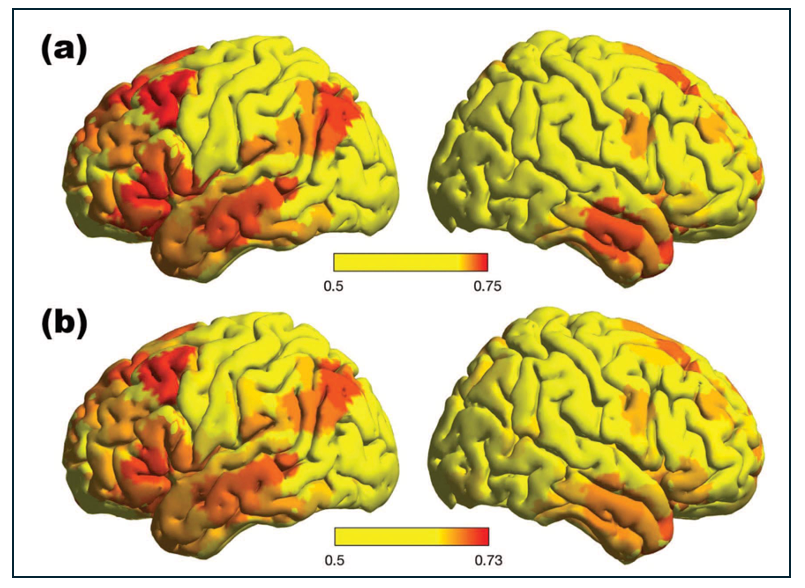
\includegraphics[width=\linewidth]{sex_classification.png}
  \caption{ROI-based sex classification shows high accuracies for (a) within sample CV and (b) across sample classification.}
  \label{fig:sexclass}
\end{wrapfigure}
and then infer which brain networks contribute most to distinguishing females from males.
\par\vspace{-1\parskip}\noindent
Our own ML work identified regionally specific networks with predictive power strongest in higher-level regions 
for language, social cognition, and emotion processing 
\parencite{weisSexClassificationResting2020a,wierschAccurateSexPrediction2023a,wierschSexDifferencesBrain2021a}.
However, RS primarily reflects intrinsic, trait-like brain organization. \\
What remains largely unexplored are 
sex differences in the “brain in action” when engaging with complex, multimodal input resembling real life. 
The present proposal aims to contribute to closing this gap in knowledge by applying the newly 
emerging NV approach to examine sex-specific brain responses in ecologically valid contexts. 
NV focuses on 
cognitive processes in dynamic, temporally extended, naturalistic contexts, which are much more akin to
situations which the brain must deal with in real life.
Importantly, as opposed to RS, all participants are exposed to the same stimulus, for which content and timing 
is known and can be used in the analyses.
NV approaches offer complex, dynamic and ongoing stimulation similar 
to experiences in everyday situations, where low-level (audiovisual) and high-level (cognitive and emotional) 
content vary fluidly, creating a multimodal and immersive experience 
\parencite{sonkusareNaturalisticStimuliNeuroscience2019}, offering the 
opportunity to capture dynamic neural processing in ecologically valid contexts 
\parencite{vanderwalMoviesMagnetNaturalistic2019} and has been shown to enhance reliability and 
identifiability compared to RS \parencite{krollNaturalisticViewingIncreases2023}.\\
Our lab has pioneered NV analyses. We developed the Topography-based Predictive Framework (TOPF) 
\parencite{liTopographybasedPredictiveFramework2023a}, which extracts individual-specific evoked 
topographies and links them to behavior using ML. 
Applied to NV data, TOPF achieved up to 80\% accuracy in 
sex classification, with predictive regions tied to emotion, language, and higher cognition. 
These promising results highlight the potential of NV to uncover novel sex differences.\\
Surprisingly, to our knowledge, no study has yet used NV to systematically examine sex differences. 
In a previous publication \parencite{eickhoffClinicalApplicationsMovie2020a}, we have compared the potential of 
movies for the study of 
individual brain differences to a cardiac stress-test, 
i.e. to potentially provide a standardized way to study the whole organ while it works to compare function 
across different levels of intensity and demands. 
We therefore expect NV to expose sex differences across a wide range of real-life-like situations—social interactions, 
face and emotion perception \parencite{sonkusareNaturalisticStimuliNeuroscience2019}, 
or complex narratives—that TB or RS approaches cannot capture. 
While isolated cognitive processes as examined in TB fMRI might not reveal 
significant sex differences, the complex interplay of these processes - as engaged during movie watching - could 
highlight more pronounced differences between women and men. 
Careful stimulus annotation will further allow us to identify the specific features and networks driving these differences.\\
Using advanced neuroimaging and analysis methods, we aim to detect subtle but meaningful sex-related differences 
in brain activity and FC, that can inform our understanding of 
broader cognitive and behavioral differences between females and males. 
First, we will study FC patterns that emerge over several minutes of movie watching. Then, we will zoom in to
identify specific events that trigger differences between women and men, and examine how these differences 
unfold in brain networks over time.\\
This multi-layered approach — combining aggregated and time-resolved FC, network dynamics, and brain activity — offers 
a richer view of sex differences in the brain function. 
Results from the proposed project can shed new light on why cognitive and behavioral patterns differ 
between women and men, and why certain neurological and psychiatric disorders present differently across the sexes. 
Such knowledge may improve diagnostic precision and personalized treatments, and support sex-specific 
strategies in healthcare and education.\\
We are uniquely positioned to realize this project, as our lab has already acquired the Ju-MOVIES dataset, 
a rich NV fMRI resource with over 130 participants. It combines extended movie stimuli, 
hormone measures, and detailed scene annotations, providing an unparalleled foundation for 
uncovering sex differences in the brain.\\
For clarity, throughout this proposal “sex” refers to self-reported biological sex. 
We acknowledge that “gender identity”, i.e. the 
subjective identification of an individual as female, male, or one of the other gender identities which might 
be also fluid, also plays a significant role, but this lies 
beyond the scope of the present project.

\subsection*{Data: The Ju-MOVIES dataset}
The proposed work builds on the Ju-MOVIES dataset, which has already been acquired and is 
uniquely suited for investigating sex differences with a NV approach. Its richness and design make it an ideal foundation for the present project. 
Over the course of the project, further data will be collected.
The paradigm comprises seven Hollywood movie excerpts (8 - 10 minutes each) selected to capture diverse social 
interactions, complex situations, and evolving emotions (“Dirty Dancing”, “Scream”, “Dead Poets Society”, “Forrest Gump”, “Dead Man Walking”, “Life is Beautiful”, 
“The Good, the Bad, the Ugly”), as well as 12 shorter clips and two RS scans of about 9 minutes. \\
Stimuli were chosen to be long enough for participants to grasp the context and empathize with characters, 
ensuring ecological validity.\\
So far, data from 135 healthy participants (68 males, 18 - 35 years) have been collected on a 3T Siemens Prisma scanner
with a 64-channel head coil, using a T2w multiband echo planar imaging sequence with the 
following parameters: repetition time (TR) = 980ms, echo time (TE) = 30ms, flip angle = 70°, field of view 
(FOV) = 207 x 207mm, voxel size=2.2 x 2.2 x 2.0mm3, number of slices: 64, multiband acceleration factor=4, 
phase encoding direction=AP,  FoV=207mm). A mirror fixed on the head coil allows participants to see a screen used 
to display the movies. In-ear headphones are used for ear protection and to deliver the movie sound. 
Additionally, a structural T1w image is acquired using an MP-RAGE sequence (TR=2000ms, TE=2.45ms, TI=900ms, 
flip angle=8°, FoV: 256mm) yielding 1mm3 voxels.\\
Alongside fMRI and structural imaging, saliva samples were collected and analyzed for levels of 
cortisol, estradiol, progesterone, and testosterone to account for hormone-related variability. 
\begin{wrapfigure}{r}{0.3\textwidth} % r = rechts, l = links
  \vspace{-10pt} % optional: kleine Korrektur, damit es bündig startet
  \includegraphics[width=\linewidth]{emotions_DMW_edited.png}
  \caption{Exemplary emotion annotation for one of the movie stimuli..}
  \label{fig:dmw}
\end{wrapfigure}Oral contraceptive use was documented in women.
The movies are richly annotated: 
emotion ratings from 44 additional participants (23 males, age 20-30 years)
for the six basic emotions (happiness, fear, surprise, sadness, disgust and anger \parencite{ekmanConstantsCulturesFace1971a}), 
sampled at 10 Hz confirmed that the stimuli evoke a wide spectrum of affective states. 
Further annotations by two indpendent raters include scene content: faces, bodies, male / female presenting characters, ethnicity of characters, presence of children, 
adults, crowds, hands, buildings, vehicles, food, landscapes, animals, plants, movement, social interactions, 
place (inside or outside / urban vs. non-urban), time of day (day or night), weather, presence of music and 
camera movements, enabling fine-grained mapping of movie features to neural responses.
Altogether, Ju-MOVIES offers a rare combination of naturalistic stimulation, hormone measures, 
and detailed scene-level annotations, providing an exceptionally strong basis for the proposed project.


\subsection*{Work Program and Research Methods}
The overarching goal of the proposed project is to complement existing research on sex differences in the brain by 
employing a NVapproach. This method promises new insights into sex differences in brain responses to complex, 
dynamically evolving situations—much closer to the demands the brain faces in real life. Our results can go beyond 
findings from both TB and RS studies and provide perspectives that previous approaches could not achieve. 
Specifically, we will identify which types of complex situations depicted in the movie stimuli give rise to the 
most pronounced sex differences. In subsequent steps, we will disentangle which narrative events within the 
movies drive these differences and examine how female and male brains respond differentially to the evolving storyline. 
We expect that this innovative approach, combining analyses of temporally aggregated 
FC, event-related responses, network dynamics and brain activity will yield important new insights into 
the multi-faceted spectrum of sex differences in the brain in action.\\
\textbf{WP1}will extend existing RS findings by examining sustained FC during NV across time periods of several 
minutes. Using a temporally aggregated FC approach, as commonly applied to RS data, this work will identify 
sex differences in “action brain states” and their underlying networks.\\
\textbf{WP2} will build on this by employing a time-resolved FC approach to detect temporally specific events 
that drive sex differences in the experience of complex situations. Leveraging detailed annotations of the 
movie content, we will characterize which types of situations give rise to pronounced sex differences and 
reveal sex-specific cognitive strategies in processing them.\\
\textbf{WP3} will focus on brain activation patterns rather than FC. Here, we will extract typical female 
and male brain responses within each brain region to the dynamically evolving movie content. This analysis will 
complement WP1 and WP2 by providing a direct account of how women's and men's brains differentially respond 
to unfolding narrative events.

\subsection*{WP 1: The Brain in Action - The Naturalistic Viewing Action State (NV-AS) }
Several studies have shown that sex classification based on RS FC can achieve high classification accuracies 
\parencite{casanovaCombiningGraphMachine2012a,ritchieSexDifferencesAdult2018, weisSexClassificationResting2020a,wierschAccurateSexPrediction2023a,wierschSexDifferencesBrain2021a} 
by capturing temporally aggregated FC patterns evoked over a sustained state of free thought or mind wandering. 
Since these RS brain patterns are independent of any external stimulation, they are often taken as a proxy 
for intrinsic brain organization, and in that sense, constitute more of a trait rather than an actual state.\\ 
The present WP aims to supplement existing results on sex differences in the brain by examining temporally 
aggregated FC patterns induced by the complex narratives presented in the movies. In contrast to RS, 
we expect movie induced brain patterns to represent states that are strongly dependent on the content of the movies. 
As this content is known, it can be used to characterize evoked FC patterns and sex differences between them. 
Thus, in this WP we will consider sustained brain “action states” (ASs) evoked by different movies and 
compare sex classification accuracies based on different naturalistic viewing ASs (NV-ASs) to RS. 
Since sex differences in NV-ASs depend on movie content, annotations the content will be employed to 
characterize the evoked brain NS-ASs and sex differences between them. 
Thus, this WP will provide insights 
into which kind of situations evoke particularly prominent differences between females and males. Here, we are 
looking at sex differences in the overall experience of complex situations, which is different both from TB 
studies looking at sex differences within specific cognitive tasks and from RS which mostly reflects intrinsic 
brain organization. We assume, that putting the brain into action while experiencing different complex situations 
should bring out differences between females and males more strongly than unrestricted and thus uncontrolled 
free thought can \parencite{vanderwalIndividualDifferencesFunctional2017}.\\
To compare enduring NV-AS to RS and amongst different movies, we will employ a similar approach as 
in our previous work \parencite{weisSexClassificationResting2020a}.\\ 
Briefly, after parcellating the fMRI data into non-overlapping parcels based on an established parcellation 
(e.g. \parencite{schaeferLocalGlobalParcellationHuman2018}), 
a mean activation time course will be computed for each parcel and correlated with those of each of the other parcels. 
Then, for each parcel individually, the FC pattern with the rest of the brain will be used as features 
to train a sex classifier for which classification accuracy will be determined by use of a cross validation (CV) 
approach. This procedure results in a spatial map of sex classification accuracies across the brain for RS and each 
NV-AS (i.e. each movie). Importantly, and in contrast to the majority of previous studies, 
we will include hormone levels and OC status in women as confounds into all prediction analyses in WP1 to 
ensure that results delineate actual differences between the sexes, rather than hormone related variability. 
In doing so, we will take particular care to control for confound leakage \parencite{hamdanConfoundleakageConfoundRemoval2022a}, 
which might bias results of the prediction analyses. 
\subsubsection*{WP 1.1:  Comparing sex classification accuracies between RS and NV-ASs}
As a first step, within each parcel, sex classification performance (across CV folds) will be compared between RS and 
NV-AS (averaged across all movies) by use of corrected resampled t-tests \parencite{nadeauInferenceGeneralizationError2003a}. 
Higher classification accuracies during NV (compared to RS) will reveal cognitive sex differences 
that are specific to the brain in action rather than to its intrinsic organization. In addition, the spatial distribution of 
highly discriminative parcels in NV will highlight the brain networks underlying these sex differences in the NV-AS. Cognitive domains 
related to the identified brain networks can be characterized by use of functional decoding \parencite{foxMetaanalysisHumanNeuroimaging2014a}. 
While sex differences 
have often been reported in the DMN for RS \parencite{weisSexClassificationResting2020a,zhangFunctionalConnectivityPredicts2018}, 
for NV-AS, we expect sex differences in higher 
cognitive or task-general networks \parencite{hugdahlExistenceGeneralizedNonspecific2015a}. Furthermore, we expect sex classification 
based on NV-AS to outperform RS, as similar effects have been observed for other phenotypes 
\parencite{finnCanBrainState2017a,vanderwalIndividualDifferencesFunctional2017} and NV has been shown to increases individual 
identifiability over RS \parencite{krollNaturalisticViewingIncreases2023}. 

\subsubsection*{WP 1.2: Which movie features drive sex classification accuracies?}
To further examine which kinds of complex situations maximize sex differences in the brain, we will characterize each movie 
clip by several visual and auditory features across the duration of the movie clips. These will comprise 
low-level features like mean motion energy, visual brightness and auditory loudness, high-level features 
like number of faces, social interactions and words, 
which can be automatically extracted \parencite{mcnamaraDevelopingComprehensiveFramework2017a,radfordRobustSpeechRecognition2022}, 
and further movie features that have been acquired in our annotations. We will then compare sex classification 
accuracies across the whole brain between the eight different movies clips by use of a multiple regression approach, 
which will delineate which movie features drive classification performance for each brain parcel. 
As higher classification performance indicates more pronounced differences between the sexes, this procedure will 
result in a “movie feature profile” explaining which features of the movies result in most pronounced sex differences. 
By clustering brain parcels according to their movie feature profiles, we will identify brain networks in which sex 
differences are conjointly driven by specific features of the movies. We hypothesize that certain brain 
networks will comprise specific cognitive domains, in particular those that have been identified in 
classical group studies, which identified sex differences in cognitive domains like language and spatial 
cognition \parencite{halpernSexDifferencesCognitive2000a,kimuraSexCognition2000a}. 
Other networks can be expected to comprise more generalized and 
non-specific cognitive resources which are independent of the specific situation \parencite{hugdahlExistenceGeneralizedNonspecific2015a}. 
We expect domain-specific brain networks to overall achieve higher sex classification accuracies than 
domain-general networks. In an exploratory approach, we will compare the expressions of these networks 
in females and males by computing the first principal component of network FC patterns in females and males separately, 
thus identifying the “typical” female and male brain network pattern for each movie feature cluster. 
An exploration of these sex specific movie feature networks should help elucidate sex specific 
cognitive strategies in response to complex life-like situations.\\ 
\textbf{Main Goal: Characterize sex differences in the NV-AS to reveal situationally modulated sex differences 
that may not be evident in RS.}\\
\textbf{Open Question: Will sex specific movie feature networks differ systematically, 
and what do these differences suggest about sex-specific cognitive strategies?}

\subsection*{WP 2: Going dynamic: Sex differences in time-resolved FC}
WP 1 will provide insights into sex differences in the overall NV-AS induced by different movies, thus
identifying sex differences in brain networks evoked over the temporally aggregated state of perceiving a
complex situation. However, one of the main advantages of using movies in the study of individual
differences is that their content varies dynamically and that due to the shared stimulus experienced by all
participants the impact of the dynamic movie content on the brain can be directly analyzed. Making use
of this, the present WP will further disentangle the temporally aggregated FC pattern of the NV-AS into
time resolved FC patterns at each time point of the movie. Going beyond characterizing “state type” movie
content as a whole, here the main aim is to directly identify specific events within the movies that result in
distinct time-point specific FC patterns that differ between females and males. These, in turn, can be further
analyzed through the use of temporally resolved rather than movie wide annotations.\\
To achieve this goal, we will again parcellate the fMRI data and compute a mean activation time course for
each parcel. Instead of considering the NV-AS, we will now decompose static FC patterns into moment-by-
moment, single repetition time (TR) co-fluctuation patterns \parencite{betzelLivingEdgeNetwork2023a,faskowitzEdgecentricFunctionalNetwork2020a}.
Basically, the Pearson correlation which is above used as a measure of temporally aggregated FC between
pairs of brain regions is “temporally unwrapped” by calculating the element-wise product of each pair of
nodes' z-scored time series. For each edge, i.e. connection between two brain parcels, this results in a time
series - typically referred to as "edge time series" (eTS) - representing the instantaneous co-fluctuation
magnitude between the pairs, or simply speaking, the development of FC over time \parencite{betzelLivingEdgeNetwork2023a}.
To identify dynamic FC differences between females and males during movie watching, we will identify
time points within the movies, at which females' and malesÄ FC patterns are most distinct. To do so, we
will employ a ML approach at each time point to classify sex based on the individual time resolved FC
patterns. Given that the dimensionality of these features, i.e. the number of edges, is extremely high, we
will first employ a principal component analysis (PCA) for dimensionality reduction. Then, for each time
point, the first n (e.g. 50) principal components will be used as features to train a sex classifier for which
classification accuracy will be determined by use of a CV approach. Again, hormone levels and OC status
will be included in the models as confounds to control for hormone related variability and possible confound
leakage will be assessed and controlled for \parencite{hamdanConfoundleakageConfoundRemoval2022a}.\\
Using permutation tests we will identify those time points, for which classification accuracy differs
significantly (p < 0.05) from chance, thus identifying events within each movie for which female and male
time-resolved FC differs most. This approach offers the unique opportunity to link temporally specific sex
differences in FC to movie content, thus identifying specific situations to which the sexes react differently.
To characterize these situations, annotations of the movies will be used to identify movie events driving
sex differences in time specific FC together with sex specific FC patterns driven by these features. To this
aim, for each of the significantly different time points, the presence or absence of specific movie features
(e.g. human bodies, faces, animals, scene cuts) will be coded binary, while continuous features (like
luminance and audio level) will be coded as continuous numbers, thus creating a movie feature vector for
each significant time point. We assume that typical sex differences in time resolved FC patterns will repeat
across similar types of scenes in the different movies. Therefore, we will cluster the time points inducing
significant differences between females and males according to their feature vectors, thus revealing parts
of the movies that evoke sex difference during scenes with similar content. Then, for each of the time point
clusters, we will compute a typical female and male FC pattern as the first component of a PCA across the
FC patterns assigned to this cluster. This will identify typical female and male FC patterns in response to
movies content associated with this cluster of movie scenes.\\
Finally, we will identify the pattern of brain regions that are most strongly involved in the typical female
and male FC patterns for each cluster. Firstly, we will threshold the typical female and male FC patterns to
identify most important edges in the sex-specific networks. Then, for each brain region, we will compute
the weighted sum of all edges connected to that region and identify most important network nodes by
selecting those for which summed FC strength exceeds the mean + 2 standard deviations across all nodes.
This procedure will identify the sex specific spatial distribution of brain networks evoked by specific scenes
in the movies.\\
Altogether, this procedure will shed light on which features within the movies induce most pronounced
differences between females and males. Together with a set of features describing the movie scenes, we
will identify female and male typical brain networks responding to these situations. While we expect to
identify cognitive domains that match those identified in classical TB studies, the present approach will not
only identify differences in specific isolated cognitive domains but reveal sex differences in cognitive
strategies of dealing with certain complex situations. For example, while TB studies have identified sex
differences in specific brain regions (like the fusiform face area) when participants viewed pictures of faces
presented in isolation, our approach will depict sex differences in the brain when faces are encountered in
a multimodal situation like in real life. Consideration of the brain networks evoked differently in females
and males will shed light on sex specific neuronal patterns in perceiving faces.\\
\textbf{Main Goal: Identify temporally specific movie events driving sex differences in the experience of real life-
like stimuli and related differences in time-resolved FC patterns.}\\
\textbf{Open Question - Relation to Classical Findings: How do naturalistic sex differences observed here relate
to findings from traditional TB paradigms (e.g., isolated face viewing)? Are the same brain regions
implicated, or do new networks emerge under ecologically valid conditions?}

\subsection*{WP 3: Shared but unique: Examination of the sex specific shared response to dynamic emotions}
One of the main advantages of NV paradigms over the RS approach is that all participants are exposed to
the same stimulus, resulting in a synchronization of the neural response across participants. However, at
the same time, substantial individual differences within this 
response are preserved \parencite{finnIdiosynchronySharedResponses2020a,vanderwalIndividualDifferencesFunctional2017}. 
In this WP, instead of looking at time resolved FC patterns, we will focus directly
on the evolution of the neural response over time to examine in more detail, whether and how females' and
males' brains differ in response to the dynamic movie content. Considering that sex differences in emotion
perception and regulation have often been suggested in the literature 
(e.g. \parencite{domesNeuralCorrelatesSex2010a,gardenerSexDifferencesEmotion2013a})
and that movies are particularly effective in inducing strong negative and positive emotions
\parencite{grossEmotionElicitationUsing1995,westermannRelativeEffectivenessValidity1996}, we will 
focus on the sex differences in the brain's reaction
to the evolving emotional content over the course of the movies' narratives. Results from this WP will
extend existing findings on sex differences in emotion perception which have mostly only focused on single
emotions in rather artificial situations.\\
To do so, we will employ the new analysis approach (TOPF, \parencite{liTopographybasedPredictiveFramework2023a}) 
which has recently been developed in our lab. Simply speaking, for each brain region, this
methodological approach extracts the
shared brain response time course across a group of participants (through use of a PCA), which is evoked
by watching the movie. Furthermore, the individual expression of this shared response is computed, which
indicates to what extent the individual brain reaction matches the typical brain response across the group.
In the present context, we will employ an adjusted “two group” version of TOPF. Instead of identifying the
shared brain response across all participants, we will identify typical brain responses for females and males
separately. Importantly, to control for hormone related variance within the data, we will regress each
subject's time series on their hormone levels and use the residuals, i.e. the part of the signal not explained
by hormones, for computation of the shared response.
For each brain region we will compare the typical female and male response in two steps: Firstly, we will
check whether the typical female response is significantly different from the typical male response. This
will identify brain regions, in which the evoked brain response to movie differs fundamentally between
females and males. To further explore whether depicted emotions are the driving factor in differential brain
activation patterns in females and males we will employ the existing emotion annotation of our movies with
respect to the six basic emotions. For each of the brain regions which display significantly different time
courses for female and males, we will correlate the female and male time course with the emotion
annotation to find out which emotions drive the differences. High correlation between the female
respectively male shared response and annotation of specific emotions will identify emotions within the
movies that drive sex differences in certain parts of the brain.\\
For brain regions, where the overall sex specific brain responses do not differ significantly, we will compare
the individual expressions of this response by a two-sample t-test. This will identify brain regions, which
react to the narrative of the movie in a similar way, but in which the intensity of the experience differs
between females and males. We expect to find both types of regions mainly in higher cognitive regions,
which we will further explore through the use of functional decoding \parencite{foxMetaanalysisHumanNeuroimaging2014a}.
Finally, we aim to find out whether, across the whole brain, females and males differ fundamentally in their
perception of the evolving narrative of the movies. To this aim, for each subject, we will compute the
similarity of individual brain response to the sex-specific typical response for each brain region. Then we
will calculate a summary score (over all regions) to determine the sex of the subject by assigning them to
the class with the higher overall similarity score. If this classification works with high accuracy, it can be
taken to indicate, that there are typical female and male whole brain patterns in the perception of complex
narratives. Should this not be the case it would speak to the brain patterns being driven by individual factors
over sex.\\
\textbf{Main Goal: Identify sex-specific patterns in neural responses to dynamic emotional content during NV,
revealing how females and males process emotionally charged situations differentially.}\\
\textbf{Open Question 1 - Which Brain Regions Show Fundamental Sex Differences? Which brain regions
exhibit fundamentally different time-resolved responses to emotional content between females and males,
and are these differences consistent across movie narratives?}\\
\textbf{Open Question 2 - Which Emotions Drive Neural Divergence? Are specific emotional categories (e.g.,
fear, anger, happiness) more likely to induce divergent neural responses between females and males?}\\




\printbibliography

\end{document}
